\subsection{Design}
\label{sec:design}

In this section we describe the design of the cloud environment and
analytics engine, we justify our design decisions in
Section~\ref{sec:justification}. Figure~\ref{fig:design-cloud} shows
the design of the cloud environment integrated with the existing
infrastructure. For more details about underlying networking and
existing network infrastructure see Appendix~\ref{app:packstack-config}.

The cloud infrastructure is built on top of the bare metal machine
described in Section~\ref{sec:hardware} and runs in a Red Hat Enterprise
Linux environment. To access the analytics platform, users must be logged into
the Oscar Proxy and then they can SSH into the host machine or guest VMs
running in the OpenStack PackStack deployment.

\begin{figure}[H]
  \centering
  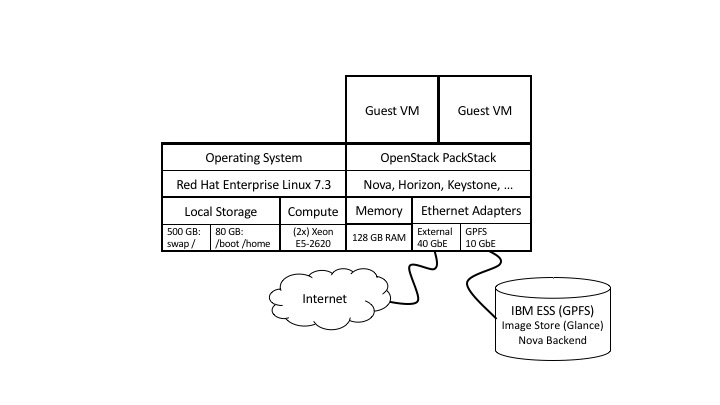
\includegraphics[scale=0.60]{img/design-cloud}
  \caption{Overview of the OpenStack deployment configuration integrated with
  the existing hardware environment.}
  \label{fig:design-cloud}
\end{figure}

Using the OpenStack deployment described above, we designed an analytics
engine following the guidelines by Meaghan Johnson~\cite{alchemy}. The
analytics engine consists of two virtual machines, the first being a
development machine (dev for short) and the second being a database
machine (db for short). The dev machine is contains all the data input
and data processing packages and tools and the db machine contains the
storage for both structured and unstructured data. The two VMs are
connected over the private internal LAN made for the OpenStack tenant as
described in Appendix~\ref{app:packstack-config}. 

\begin{figure}[H]
  \centering
  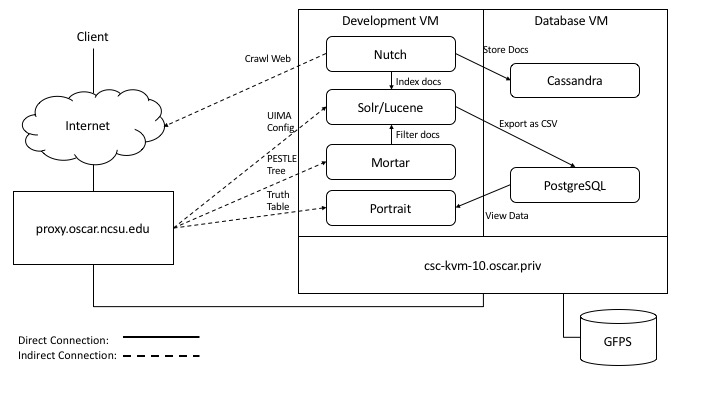
\includegraphics[scale=0.60]{img/design-workflow}
  \caption{Overview of the workflow for data analysis in the
    implemented data analytics engine. *This figure is adapted
    from the document and presentation by Meaghan Johnson}
  \label{fig:design-workflow}
\end{figure}

Figure~\ref{fig:design-workflow} shows the design of the analytics
engine and contains a sample work flow of the system. The dev machine
contains Nutch for data input, Solr for structuring data, Mortar for
filtering data, and Portrait for visualizing data. The dev machine is
connected to the db machine which contains Cassandra for storing
unstructured data and a PostgreSQL database for storing structured data.
Once again these machines are connected via private internal LAN.\\

\mypara{Sample Workflow} To use out data analytics engine users
interact with the system in the following way:

\begin{enumerate}[Step 1.]
  \item User logs into oscar proxy via SSH
  \item User sends an URL file to dev
  \item User logs into dev and injects the URLs into Cassandra from the
    command line
  \item User creates a batch file from the injected URLs from the
    command line
  \item User crawls the web using the generated batch file with Nutch
    from the command line
  \item The user updates Cassandra with the results from the command
    line
  \item The user indexes the results with Solr from the command line
  \item The user develops an annotator locally and copies the jar to dev
  \item The user logs in to the Mortar interface and filters the data in
    Solr
  \item The user installs the annotator on Solr from the command line
  \item The user updates the Solr indexes from the command line
  \item The user imports the structured data from Solr to the PostgreSQL
    database from the command line 
  \item The user visualizes and queries the structured data using the
    Portrait user interface
\end{enumerate}

During the design of the analytics platform and analysis engine we
discovered the following best practices:

\begin{itemize}
  \item \textbf{External Storage Devices}

     In this project we discovered how to attach external storage
     devices and how to configure them to be used to store Glance images
     and the back end for Nova instance. This best practice can be
     leveraged to subvert small local disks on compute nodes.

  \item \textbf{``Double NAT public IP address'' }

     We discovered it is possible to route traffic to guest VMs by
     assigning it an IP address from the OpenStack external network. In
     the absence of public IP space, it is possible to bridge the external 
     network to the existing network and assign the guest a private IP 
     address to act like a public address. 

     One additional step can use port forwarding on the public IP
     address of the host machine to make the guest truly routable from
     the Internet but we did not have administrator privileges on the 
     proxy with the public IP address.

  \item \textbf{Image Versioning}

     A best practice that proved itself useful many times was creating 
     image snapshots during image development. Before performing 
     development steps that could have a major impact on the system, we
     took an image snapshot and if the changes created an unstable image
     we could safely and quickly revert the image back to a consistent
     state and begin development again.

\end{itemize}


The rest of this section details how our design addresses the issues
identified in Section~\ref{sec:issues}.

\subsubsection{Security}
\label{sec:security}

As mentioned in Section	\ref{sec:issues} security is one of the greatest
concerns of consumers when considering the transition to the cloud. In our
design, security comes up in a number of different places. When we
consider a design decision and its implications on security we used
the following threat model to properly assess the risk and impact of that
decision.\\

\mypara{Threat Model} We assume an adversary external to the network,
without physical access to the host machine or a privileged account to
the host machine, the guest VMs, or the Oscar Lab proxy. Furthermore,
the adversary is not an administrator or other insider working for the
client or provider. It is assumed the adversary has the necessary skills
and resources to remotely discover and exploit vulnerabilities on a system
to gain unauthorized access to machines. Once the adversary obtains
access they can exploit more vulnerabilities on the system resulting in
local privilege escalation. Finally with local privileges the adversary
has the goal of exfiltrating sensitive data from the host.

Under this threat model we identify two components in the attack
surface, the Oscar Proxy and the Nutch web crawler. Since the host
machine and guests are not reachable via public Internet, all users must
authenticate with the Oscar Proxy to obtain access to use the platform.
Thus the security of the system relies upon the security of the proxy.
Control of the proxy, and thus the ability to completely assess the
security, was not given for this project; however, we note the following
practices currently in place for access control to the proxy. Currently,
access is delegated from a trust system administrator in the Oscar Lab
to a client. The client's account may only use RSA private key
authentication and password-based authentication is disabled. We
recommend following this best practice, with proper least privilege to
user accounts on the proxy and key sizes of at least 2048 with key sizes
4096 recommended. Further we recommend minimalistic services on the
proxy and continuous security updates. As a fail safe we have the
following security measures:

\begin{enumerate}
  \item \textbf{Isolation} the guest VMs are physically isolated from the
proxy thus the adversary must launch another attack after compromising
the proxy.
  \item \textbf{Guest Access Control} password authentication is
disabled on the guests protected by a second RSA key. Further, guests
only allow incoming traffic from the host machine and the proxy. This
could be further locked to only allow traffic from the host, but for
usability we allow traffic from the proxy.
  \item \textbf{OpenStack Access Control} since the web interface does
not support key based authentication, we implement access control to the
horizon interface via a randomly generated password.
\end{enumerate}


The second component in the attack surface is the Nutch web crawler. The
only way to communicate with the system is via the proxy (discussed
above) and by hosting data on a web page crawled by Nutch. The security
of Nutch is out of scope for this analysis but the compromised guest
cannot interact with other tenant machines or the host machine, with
mechanisms in place by OpenStack, although rare vulnerabilities have
allowed such attacks in the past. We leave protection of these severe
attacks to be addressed by OpenStack developers.

\subsubsection{Portability}
\label{sec:portability}
Following security, portability is one of the next biggest issues
consumers face when exploring the transition to the cloud. The first
concern is whether their current environment can run in the cloud with
little to modification and they also consider they ability to export
their environment from the cloud when they are done.

This system addresses the issue of portability in a very simple and
straight forward manner. Our OpenStack deployment is backed by a
hypervisor with libvirt and QEMU support. Thus users can create virtual
machines locally that run on their own libvirt hypervisor and import
them into our environment or they may download the image and run it
locally in their environment. QCOW2 image formats are widely supported
and users wishing to move to a cloud that does not support the QCOW2
format may convert their image using popular open source image
converting tools.

\subsubsection{Structuring Data}
\label{sec:structuring}
How to handle and operate on unstructured data is huge issue as data
collection rates increase faster than the ability to define a structure
for it. Although this issue is something that does not need to be
addressed by all data analysis platforms, our analytics engine
specifically takes unstructured data as input and must convert it to
structured data before combining it with existing structured data and
finally analyzing it.

Our system directly supports the storage of unstructured data in
Cassandra, once the unstructured data is collected users may interact
with the data in Solr to apply filters and annotators to structure the
data. Once structured the data is then stored in a PostgreSQL database
which can be visualized by the user. The Solr component is well known
and used tool which should be familiar to the user.


\subsubsection{Ease of Use}
\label{sec:ease}
The final issue mentioned in Section~\ref{sec:issues} is Ease of Use or
the Usability of the platform. If a consumer is going to pay for a
product, they expect the product to be robust, easy to use, and well
documented. However, it is hard to precisely measure the usability of a
product and we evaluate our system on its ability to provide nice
graphical user interfaces when possible and minimize command line
interaction and configuration.

In our design users can access the Horizon web interface for deploying
and managing virtual machines, the Solr web interface for managing and
indexing data, and the mortar/portrait interface for filtering and
visualizing the data. Components that require command line interaction
are popular well documented tools and it is assumed the user is
familiar with these components already. Finally the data analysis engine
is comprised of two VMs which are preconfigured, however if the user
needs to reconfigure the guest VMs to talk to each other they only need
to change the peer IP addresses of the components in a few files.

The first set of components that need to communicate with each other are
Nutch on the dev machine and Cassandra on the DB machine. On the dev
machine in /opt/nutch/conf/gora.properties set:\\
\textit{gora.cassandrastore.servers = IP:PORT}\\
and in /opt/nutch/conf/gora-cassandra-mapping.xml set:\\
\textit{$<$keyspace name=``webpage'' cluster=``Test Cluster''
host=``IP''$>$} and\\
\textit{$<$keyspace name=``host'' cluster=``Test Cluster''
host=``IP''$>$}

Finally to configure Nutch and Cassandra modify 
/opt/cassandra/conf/cassandra.yaml on the DB machine to have the
following lines:\\
\textit{seeds: ``IP''\\listen\_address: IP\\start\_rpc:
true\\rpc\_address: IP}

After these changes, Cassandra and Nutch are configured to communicate
with each other. The other set of components that need to communicate
are Portrait and PostgresSQL. The first step to allowing communication
is to allow PostgreSQL to accept connections from the dev machine. This
is done by modifying /var/lib/pgsql/data/pg\_hba.conf on the DB machine
to contain the following line:\\
\textit{host all all IP md5}

With this line PostgreSQL is now reachable from the dev machine and
Portrait can be configured to use PostgreSQL with following
modification to /opt/mortar/project/settings.py on the dev machine:\\
\begin{lstlisting}[escapechar=&]
DATABASES = {
  'default': {
    'ENGINE': 'django.db.backends.postgresql',
    'NAME': 'mortar',
    'USER': 'team1_user',
    'PASSWORD': 'team1',
    'HOST': 'IP',
    'PORT': '5432',
  }
}
\end{lstlisting}


